\begin{figure}[tb]
    \label{fig:query-time-no-snap}
    \centering
    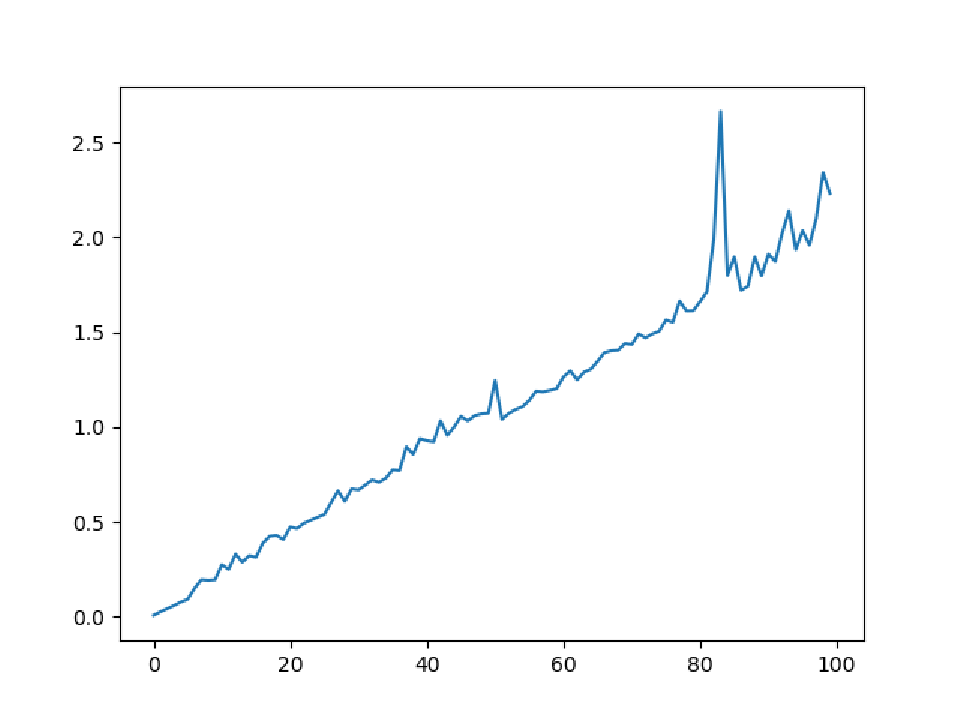
\includegraphics[width=2.8in]{figs/runtime.pdf}
    \caption{Query answering for 100 queries without snapshots.}
\end{figure}




\section{Algorithm}

We first solve the simpler single snapshot placement problem.

\begin{prop}
    \label{thm:single}
    The single snapshot placement problem can be solved in $\mathcal{O}(|T_Q|)$,
    with the optimal snapshot placement at
    $ s^*(T_Q) = \mathrm{median}(T_Q) $,
    which can be computed in $\mathcal{O}(|T_Q|)$.
\end{prop}

%\textcolor{red}{Proof [Outline]}

So by Proposition~\ref{thm:single}, it's straightforward to compute the optimal
placement of a single snapshot with respect to a given query workload.  However,
in practice, we want to allocate a number, $m$, of snapshots to be placed, where
$m$ is a determined by the available resource.
In this section, we extend Proposition~\ref{thm:single} to handle arbitrary number
of snapshots.

First we will present an recursive algorithm that solves the optimal
$m$-snapshot placement problem.

Without loss of generality, let's assume that  the query timestamps are sorted
in $Q = \{q_1, q_2, \dots, q_n\}$.  Here $Q$ is the sorted list of query
timestamps.  We denote $Q[i,j] = \{q_i, q_{i+1}, \dots, q_{j-1}, q_j\}$.

The objective is to compute $S = \{s_1, s_2, \dots, s_m\}$ such
that the query answering time given by $\mathrm{cost}(Q|S)$ is minimized.

\begin{prop}[Segmentation of queries]
    \label{thm:seg}
    Given any snapshot timestamps in a sorted order $S = \{s_1, s_2, \dots,
    s_m\}$ such that $s_i\leq s_{i+1}$, the snapshots partition the queries $Q$
    into $m$ non-overlapping segments $Q[1, i_1], Q[i_1+1, i_2], \dots
    Q[i_{m-1}, i_m]$ such that queries in $Q[i_j, i_{j+1}]$ uses $s_j$
    in the optimal query answer strategy.
\end{prop}

Proposition~\ref{thm:seg} allows us to construct a dynamic programming algorithm
that computes the {\em exact} optimal snapshot placements.

\subsection{Recursive formulation}
\label{sec:recursive}

Let $\mathrm{opt}(Q, m)$ be the optimal $m$-snapshot placements for the query
workload $Q$.

\begin{prop}[Optimality of sub-problems]
    \label{thm:subopt}
    Let $S^* = \mathrm{opt}(Q, m)$.  Let $\mathcal{Q}$ be the partition
    of segments created by $S^*$.  Then, the prefix of $S^*$ is also an optimal
    $m-1$ snapshot placement of the prefix of $\mathcal{Q}$.  Formally,

    $$\mathrm{prefix}(S^*) = \mathrm{opt}(\cup\mathrm{prefix}(\mathcal{Q}), m-1)$$
\end{prop}

We can formulate a recursive definition of $\mathrm{opt}(Q, m)$ using
Proposition~\ref{thm:subopt}.  The intuition is that we try out all possible
{\em last} segment of $Q$, and pick the one with the lowest cost.

The recursive definition of $\mathrm{opt}(Q, m)$ is given as:

\begin{itemize}
    \item Base case $ \mathrm{opt}(Q, 1) = \{\mathrm{median}(Q)\}$.
    \item Induction on $m$:
    $$i^* = \mathrm{argmin}\{\mathrm{cost}(\mathrm{opt}(Q[1,i], m-1)): i\in[1,
    n]\}$$
    $$
    \mathrm{opt}(Q, m) = \mathrm{opt}(Q[1, i^*]) \cup \{\mathrm{median}(Q[i^*+1, n])
    $$
\end{itemize}

\begin{prop}
    The recursive formulation of $\mathrm{opt}(Q, m)$ requires
    $\mathcal{O}(2^{m})$.
\end{prop}

Fortunately, we are able implement $\mathrm{opt}(Q, m)$ in polynomial time as a
dynamic programming problem.

\subsection{Dynamic programming formulation}
\label{sec:dynamic}

We can build a table $\mathbf{OPT}$ as a two dimensional array
indexed by $(i, k)$ where $i\in [1, n]$ and $k\in [1, m]$.  Each entry
in the table $\mathbf{OPT}[i,k] = \mathrm{opt}(Q[1,i], k)$.
We can compute $\mathbf{OPT}[i,k]$ in a bottom up fashion \cite{kossmann2000iterative}.

\vspace{1em}
{\small
\begin{tabular}{|l|} \hline
    computeOPT($Q$, $m$) = \\
    \verb|| $n = |Q|$ \\
    \verb|| $\mathbf{OPT}[i, 0] = \infty$ \\
    \verb|| for $k = 1 \to m$ \\
    \verb| | for $i = 1 \to n$ \\
    \verb|  | $j^* = \underset{j\in[1,i]}{\mathrm{argmin}}
                (\mathrm{cost}(\mathbf{OPT}[j,k-1]) + \mathrm{cost}(Q[j+1, n]))$ \\
    \verb|  | $\mathbf{OPT}[i,k] = \mathbf{OPT}[j^*, k-1] \cup \{\mathrm{median}(Q[j+1], n)\}$ \\
    \verb| | end for \\
    \verb|| end for \\ \hline
\end{tabular}
}
\vspace{1em}

\begin{prop}
    The complexity of computing all the entries of $\mathbf{OPT}$ is
    $\mathcal{O}(mn^2)$.
\end{prop}

